%# -*- coding: utf-8-unix -*-
%%==================================================
%% chapter02.tex
%%==================================================

%\bibliographystyle{sjtu2}%[此处用于每章都生产参考文献]
\chapter{WEB设计开发理论、技术和工具}
\label{chap:web_dev}
软件工程是研究和应用如何以系统性的、规范化的、可定量的过程化方法去开发和维护软件\supercite{radatz1990ieee},以及如何把经过时间考验而证明正确的管理技术和当前能够得到的最好的技术方法结合起来的学科。它涉及到程序设计语言、数据库、软件开发工具、系统平台、标准、设计模式等方面。所以本课题首先学习了软件开发尤其是WEB开发的相关理论,调研、比较并选择了一些主流的WEB开发技术和高效的WEB开发工具,以期能够用快速、高效、低成本地完成系统的开发。
\section{设计理论}
本系统在开发速度、可重用性、UI/UE、响应式、实时性等方面具有较高的要求,这就意味着传统的瀑布式开发、CSS+HTML、ajax请求等WEB开发理论不能达到本系统的要求。本章学习的理论可以给开发明确可行性、指明开发的方向、提高效率、减少重复造轮子,从而保证系统的顺利实现。
\subsection{敏捷开发}
敏捷开发有很多种,它们的具体名称、理念、过程、术语都不尽相同,相对于「非敏捷」,更强调程序员团队与业务专家之间的紧密协作、面对面的沟通(认为比书面的文档更有效)、频繁交付新的软件版本、紧凑而自我组织型的团队、能够很好地适应需求变化的代码编写和团队组织方法,也更注重软件开发過程中人的作用。\supercite{beck2013agile}

Clarity是一家创业公司,业务需求变化迅速,人员结构比较精简,因此更加适合用敏捷开发。本系统的软件开发团队由3个人组成,每天早晨与需求方即公司CEO和硬件开发团队进行视频通话来总结前一天的开发进度和确定当天的开发任务,不断地在测试服务器部署新特性(feature)版本和在生产服务器部署热修复(hotfix)版本,每个特性完成后再正式发布(release)到生产服务器上,团队成员吃住同行、分工灵活,每个人都能独当一面。
\subsection{Web Components}
Web Components是一组现在已经被W3C加入HTML和DOM规范的、为Web提供了一套标准组件模型的浏览器新特性,它们的设计理念是把“基于组件的软件工程”\footnote{软件工程的一个分支,是一种基于重用的定义、实现和组合松散的独立组件的软件来开发系统的方法}带到互联网的世界。Web Components主要包括4个特性:
\begin{description}
  \item[自定义元素(Custom Elements)] 定义新的HTML元素的应用程序接口
  \item[影DOM(Shadow DOM)] 兼具封装性和可组合性的DOM和样式
  \item[HTML 引入(HTML Imports)] 可声明的引入HTML文档到其他HTML文档的方法
  \item[HTML 模板(HTML Templates)] 新的<template>\footnote{\url{https://developer.mozilla.org/en-US/docs/Web/HTML/Element/template}}标签,允许HTML文档包含惰性(延后定义或加载)的DOM块
\end{description}

本系统的软件开发团队接受过良好的软件工程教育,对于重复造轮子这样的事情是坚决抵制的,所以我们对于组件的可重用性要求非常高。虽然本系统最终没有直接使用Web Components的官方实现Polymer,但其中自定义元素、HTML 引入和HTML 模板等特性都是非常有意义的,本系统中使用的Angular和React都有这些理念的原型,本系统在实现组件时也大量使用了这些概念来做到组件的可重用性。

\subsection{Material-design}
Material Design,代号为Quantum Paper\footnote{\url{http://www.androidpolice.com/2014/06/11/exclusive-quantum-paper-and-googles-upcoming-effort-to-make-consistent-ui-simple/}}, 是由Google推出的一种全新的设计语言,旨在为手机、平板、台式机等不同平台提供更加一致且广泛的外观和感觉。Material Design 总体来讲是一种隐喻式的基于纸张和墨水的设计,元素是扁平的、有阴影的,按照各自的高度浮动在背景上方,接缝和阴影让你知道哪些元素是可以触碰到的(操作的)。当你移动或改变它们的高度的时候,感觉是一张纸在被移动,符合人们对三维物体的直觉,与真实的纸不同之处在于Material Design的纸可以智能的伸缩和变形。

Clarity的CEO本人是一名正在读本科的大学生,从创业伊始就对不管是硬件还是软件要求都特别高,在UI方面尤其如此,Material Design是为数不多的能满足他的要求的设计语言。本系统中版本管理模块和Smart City模块都使用了Material Design,深受设计师、程序员和用户喜爱,因为在这套设计语言的基础上,设计师省去了很多繁琐的顾虑,程序员实现时也有比较好的UI库,界面简洁明了,让用户直观地感受到页面上不同层次不同元素的重要性。

\subsection{响应式设计 和 Flex 布局}
响应式设计是一种WEB设计方法,旨在构建出可以提供跨设备的(从桌面电脑到移动设备)拥有最佳的视觉和交互体验的网站,方便用户使用最少的缩放、平移和滚动操作来阅读和浏览。\supercite{marcotte2013responsive}为自动适应浏览者的设备环境,响应式网站使用流式的基于比例的网格布局,弹性的图片和CSS3 media queries\footnote{没有正式的中文译名,直译为媒体查询,是CSS中@media规则的扩展}做到了以下几点:
\begin{description}
  \item[流式网格] 流式网格要求页面元素按照如百分比之类的相对单位来缩放而不是传统的如像素或点的绝对单位;
  \item[弹性图片] 为防止图片显示时超出容器范围,弹性图片也按照相对单位来缩放;
  \item[Media queries] Media queries 允许页面上的元素根据显示设备的某种属性来使用不同的样式,这里的属性主要是设备的宽度;
\end{description}

Flex 布局,全称CSS Flex Box Layout,意思为弹性盒状模型布局,它是由W3C在2009年提出的一种新的布局方案,可以简便地、完整地、响应式地实现各种简单或复杂的页面布局,目前所有主流浏览器都支持Flex 布局。

Clarity作为一家创业公司没有那么多精力同时维护不同平台上的应用,因此虽然目前并不要求适配手机,但起码的屏幕宽度兼容是需要的,为将来适配更小的屏幕打好基础。本系统中三个模块都使用了flex布局,从而使得页面上的元素可以随着设备屏幕大小的变化(或浏览器的缩放)而自动伸缩。虽然我们的系统不需要适配手机,但其中版本管理模块因为页面上有比较宽的列表,在窄屏幕上显示不正常,于是采用了响应式设计来避免这个问题。
\subsection{RESTful API设计和Web Socket数据更新}
RESTful 中文名叫“具象状态传输”,全称“Representational state transfer”,它是一种包含一系列同在一个分布式网络系统中协调的组件、连接器和数据元素如何按照不同的角色进行交互的设计原则(或者叫设计风格),旨在促进系统的性能、可扩展性、简单性、可修改性、可读性、便携性和可靠性。\supercite{fielding2002principled,fielding2000architectural}相比于SOAP\footnote{Simple Object Access protocol,简单对象访问协议}和XML-RPC\footnote{XML(标准通用标记语言下的一个子集)远程方法调用}更加简单轻量,在URL处理和Payload编码上更加简洁明了。这套设计原则并不局限于WEB应用程序,只要满足其约束条件的和原则的应用程序或设计就是RESTful。WEB应用程序最重要的REST原则是,客户端和服务器之间的交互在不同请求之间是无状态的,这就意味着服务器可以随时重启并且客户端并不关心连接的是哪台服务器,这十分适合云计算\footnote{提供动态的易扩展的虚拟化计算资源的互联网服务模式}的环境。

WebSocket 是HTML5\footnote{万维网的核心语言、标准通用标记语言下的一个应用超文本标记语言(HTML)的第五次重大修改}中一种新的通信协议,浏览器与服务器通过一个TCP\footnote{即Transmission Control Protocol 传输控制协议}连接上的全双工通信(full-duplex)进行交互,只有一开始的握手需要借助HTTP\footnote{即HyperText Transfer Protocol超文本传输协议,是互联网上应用最为广泛的一种网络协议}请求完成。它使得浏览器可以和网站进行更多更频繁更实时的交互,从而可以摒弃从前通过轮询\footnote{每隔一秒向服务器发送一个HTTP请求来获取最新数据}来获取最新数据却会给服务器带来沉重负担的方法。

Clarity如其他众多创业公司一样,选择使用云服务器来搭载自己的服务,因为其自动扩展的虚拟化资源无论是直接成本还是管理成本都比自己公司搭建服务器低。本系统搭载在AWS云服务器上,无状态交互是可扩展性的一大保障,频繁地增删改查设备等数据资源也需要RESTful,于是设计了一套RESTful风格的API,前端和后端分别遵循API接口来实现。另一方面需要让用户能够实时地看到自己的修改以及空气质量的变化,本系统使用WebSocket来实时地更新数据,前后端分别使用收听和发送相关主题(topic)。
\subsection{Oauth 和 JWT}
OAuth是Open Authorization的简写,它是一个被广泛用作互联网用户使用它们的微软、Google、Facebook、Twitter等账号在不用输入它们的密码的情况下登录到第三方网站的开放授权标准。一般来讲,OAuth提供给客户端一个代表资源拥有者访问服务器资源的“安全访问授权”。它规定了资源拥有者授权第三方访问其服务器资源而无需共享它们的凭据的过程。它是专门为超文本传输协议(HTTP)设计的,本质上OAuth允许一个授权服务器在资源拥有者批准的情况下直接把访问令牌(Access Token)发送到第三方客户端,然后第三方再使用访问令牌来获取资源服务器上被保护的资源。\supercite{hardt4rfc6749}

JWT 是 JSON Web Token的简写,它是一个用来在WEB应用环境下在不同参与者之间传递声明(claims)的开放标准。这些令牌被巧妙地设计成紧凑、URL安全且可用的,最适合使用在浏览器单点登录\footnote{SSO, single sign-on}的情况下。JWT声明被典型地用于在身份提供者和服务提供者或者任何其他业务过程中需要身份的地方之间传递认证用户的身份识别。\supercite{bradley2015json}这些令牌本身也可以被认证和加密。

Clarity虽然业务规模还不大,用户数量也很少,但在安全认证方面也是紧跟行业潮流,为将来接入各种社交账号登录做准备。本系统使用OAuth标准,其中访问令牌(Access Token)使用的是JWT。用户登陆后除了会获得一个对应的访问令牌之外还有一个寿命较长的刷新令牌(Refresh Token)用来在用户短期离线后自动刷新访问令牌,而这一切除了一开始的登录都不需要用户重新输入密码,只有在用户长期离线刷新令牌也过期的情况下才需要再次登录。

除了对HTTP请求做了权限验证之外,本系统对WebSocket部分也做了相应的权限验证,socket客户端连接上Socket服务器后,会先通过socket把自己的访问令牌(Access Token)发送给服务器,服务器验证后会发回一个通过验证或者未通过验证的消息,socket客户端通过收听这两个消息来知道自己是否验证成功。如果socket客户端未通过验证,就会通知前端的原本用来刷新令牌的机制去刷新访问令牌。而每次访问令牌被改变或刷新后,socket客户端都会重新发送请求认证的消息,socket服务端也会通知客户端之前的认证已经失效。

\subsection{Flux 架构模式}
Flux 是Facebook用来构建客户端WEB应用的应用架构,它利用一个单向的数据流对React\footnote{会在下一节技术架构中介绍到}的可组合的视图组件进行了有力的补充。它更像是一种模式而不是一个框架,所以在这里本课题认为它属于理论而不是技术。

它与传统的MVC模型\footnote{即Model View Controller,是一种软件设计典范}不同,主要包括三部分:dispatcher、store和view,由action来触发状态(state)变化。如下图所示: 所有的action会进入到dispatcher进行处理,dispatcher会产生新的state用以更新store,store选择恰当的时机更新后通过view提前注册好的消息(回调)来告诉view更新用户界面。但其实大部分情况下action由用户的操作产生,因此会有从view产生的action。

\begin{figure}[!htp]
 \centering
 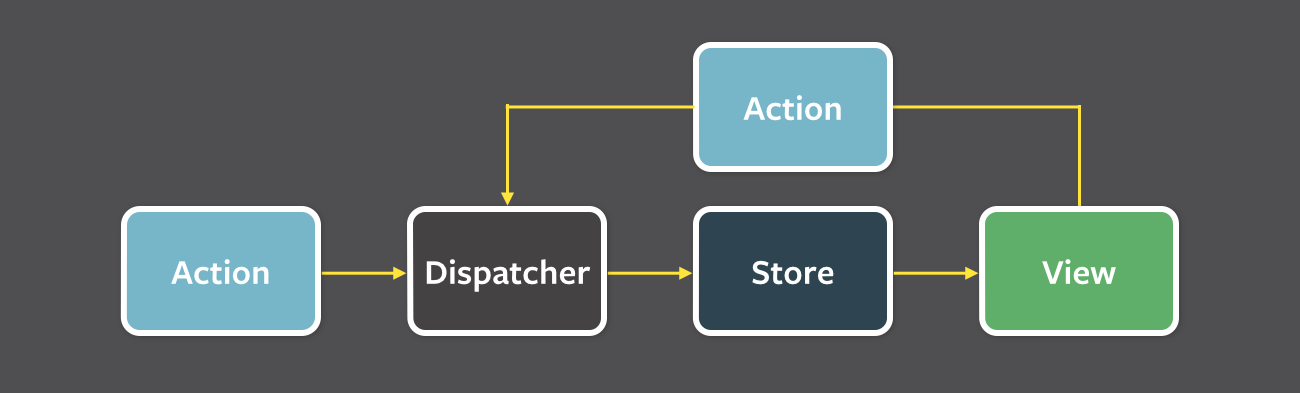
\includegraphics[width=0.9\textwidth]{flux.png}
 \bicaption[fig:longcaptionbad]{Flux 单向数据流}{Flux 单向数据流}{Fig}{Flux Unidirectional Data Flow}
\end{figure}

单向数据流传输的Flux不会像MVC那样,一旦系统复杂了,model和view之间的联系呈几何级数增长,也不会像双向绑定那样,一旦绑定层数多了,连程序员自己都不清楚状态更新是被哪里触发的。

Clarity致力于给用户最好的体验,因此在给合作方做的Smart Home和Smart City两个模块中使用了Flux架构模式。用户也许会在潜意识里感觉到,他们在我们的应用上看到的状态永远是一致的,不会出现类似明明看到有未读的消息点进去却发现没有的情况。

\section{技术架构}
Clarity的开发团队是一个精简且高效的年轻团队,我们选择了统一而不是分散的技术栈:全栈JavaScript。从前端到后端,从业务逻辑到单元测试,全部使用JS,这样给我们带来了不少好处:
\begin{enumerate*}
  \item 提高了代码重用率,因为前后端可以共同使用一些代码逻辑
  \item 提高了分工灵活度,前后端的人力可以随时支援对方
  \item 提高了开发速度,因为全栈JS的生态圈很强大、包管理系统也非常省心省力
  \item 提高了代码可维护性,因为全栈JS的各种代码规范标准非常强大\ldots
\end{enumerate*}

下面就开始分前端、后端、数据库和服务器来介绍本系统的技术架构:
\subsection{前端: Angular VS React}
目前JS的主流前端技术无外乎两个选择,Angular和React,如图2-2所示,这两个项目在Github上排行分别是第5和第6。
\begin{figure}[!htp]
 \centering
 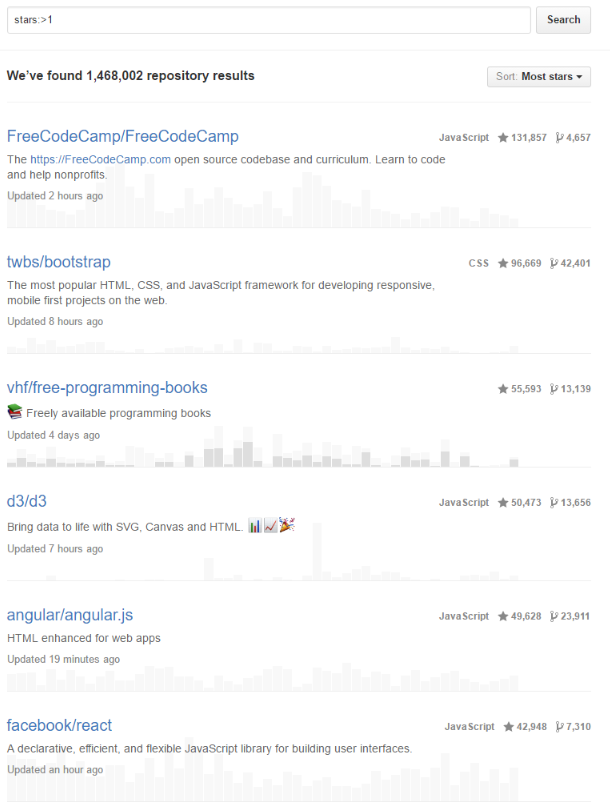
\includegraphics[width=0.9\textwidth]{github_rank.png}
 \bicaption[fig:longcaptionbad]{Github angular和react排名情况}{Github angular和react排名情况}{Fig}{Github star ranking of angular and react}
\end{figure}
\subsubsection{Angular}
AngularJS 是一个主要由Google维护的开源WEB应用框架,另外还有一个由个人和企业组成的解决SPA\footnote{Single-page applications单页面应用}开发过程中遇到的挑战的社区参与维护。AngularJS旨在通过提供一个客户端MVC架构和MVVM\footnote{model-view-viewmodel}架构的框架来简化SPA的开发和测试,另外它还提供了许多在丰富互联网应用(Rich Internet Application)\footnote{是一种拥有很多桌面应用软件特性的WEB应用 }中被广泛使用的组件(component)。

AngularJS 首先读取预先嵌入了额外的自定义标签和自定义属性的HTML页面,Angular把这些标签和属性解译为一些directive\footnote{AngularJS中对可重用组件的定义},它们可以把页面上输入和输出的部分绑定到一个标准JavaScript变量模型(model),模型中的值可以在代码中设置或者来自静态或动态的JSON\footnote{JavaScript Object Notation,是一种使用可读的文本来传输以键值对表示的数据对象的开放标准格式}资源。

AngularJS 在2010年首次发布,除了开源,它有一些创举,极大解放了前端工程师以及后端工程师的生产力:
\begin{enumerate}
  \item 使用依赖注入(dependency injection)\footnote{一种使用控制反转来处理依赖管理的软件设计模式},使得客户端也可以使用MVC,把WEB应用程序的客户端和服务端解耦合了,减轻了原本后端路由控制、页面渲染的负担,使得两边都可以被重用
  \item 使用双向绑定(two-way data binding)\footnote{视图和逻辑中的模型变量(model)互相绑定,牵一发而动全身},把DOM操作从应用程序逻辑中移除了(或者说尽量避免使用),增强了客户端程序的可测试性和性能;增强了HTML,在HTML标签中插入模型变量(model),使得开发者编写HTML时“所见既所得”。
  \item 提供了一整套构建WEB应用的过程:从UI设计,到业务逻辑,再到测试,大量的可重用组件和强大的生态圈使得开发者大量减少重复造轮子的现象
\end{enumerate}

\subsubsection{React}
ReactJS 是一个用来把视图数据渲染为HTML的开源JavaScript库,它的主要维护者是Facebook、Instagram和一个由个人开发者和企业组成的社区。React视图用以自定义HTML标签形式定义的组件(component)来渲染,这些组件可以也包含其他的组件。React在现代单页面应用开发上给开发者提供了一个这样的模型:
\begin{enumerate*}
  \item 子组件无法直接影响父组件的\footnote{所谓的数据向下流,data flows down}
  \item 当数据有所改变时,高效地更新HTML文档(document)
  \item 干净的组件隔离
\end{enumerate*}

ReactJS 是一个年轻的库,它在2011年被首次部署,在2013年美国JS大会(JSConf US 2013)上被开源,它吸收了很多Angular的优点,同时也发现了Angular的不足,总得来讲,ReactJS有以下几点特性是它如此成功的原因:

\begin{description}
  \item[单向数据流(One-way data flow)] 主要由前文介绍的Flux架构保证,每个组件会收到一些属性(properties)用来渲染到HTML标签中。与Angular的双向绑定不同,组件本身不可直接修改这些属性,只能通过作为属性传入的回调函数来修改,在Flux架构中,就是触发Action,这种原理被叫做“properties flow down actions flow up”。
  \item[虚拟DOM(Virtual DOM)] React构造了一个内存中的DOM缓存,统一计算每次渲染之间的差异,然后高效地对浏览器中的DOM进行差异更新,相比于Angular而言,Angular是监听每个视图模型(model)的变化,然后更新DOM中对应的部分,并没有差异更新的能力。
  \item[JSX\footnote{一种JavaScript的扩展语法,可以在JS代码中方便地引用HTML和使用HTML标签}] JSX允许React很方便地在JS代码中渲染子组件(subcomponents)。与Angular增强HTML不同,React依靠JavaScript本身的强大,更加方便地做到了一样的功能。
\end{description}

不得不提的一点是Angular的团队同样知道这些不足,并开发了Angular2,Angular2在很多方面与React很相似,同时又保留了一些Angular的优点。

\subsubsection{综合比较与选择}
目前来说Angular是2015年的JS宠儿,而React则后来居上,其实Angular2应当能与React媲美,但是在项目研发时,Angular2离可以正式使用还有一段距离,React则已经接近正式发布。

Angular和React最大的不同在于一个是WEB框架,一个是JS库。WEB框架意味着开发一个主流的单页面WEB应用程序所需要的一切\footnote{狭义上的,当然不包括各种开发工具}Angular都提供给你了,而React崇尚小而精,它只提供了最核心的部分,其他部分都由开发者自己从社区中选择或者自己开发组合起来搭建一个WEB应用程序。因此也就带来了Angular和React的一大不同,Angular开发WEB应用程序比较方便快捷,而用React则有更多的选择,可以有更多的个性化定制,更加灵活多变。

\begin{table}[!htpb]
  \bicaption[tab:footnote]{Angular和React的对比}{Angular和React的对比}{Table}{Comparisons between Angular and React}
  \centering
  \begin{threeparttable}[b]
    \begin{tabular}{lcr}
      \toprule
      对比 & Angular & React \\
      \midrule
      灵活度 & 一般  & 灵活多变 \\
      稳定性 & 稳定且成熟  & 接近稳定 \\
      开发速度 & 快 & 一般
      社区    & 强大  & 一般但快速成长 \\
      性能 & 一般 & 很高 \\
      支持Web Component\tnote{1} & 弱 & 强 \\
      视图核心语言 & HTML & JavaScript \\
      页面一致性\tnote{2} & 一般 & 强 \\
      \bottomrule
    \end{tabular}
    \begin{tablenotes}
    \item [1] React设计之初就考虑到对Web Component的支持,而Angular的发布和Web Component概念提出大概是在同一时期.
    \item [2] 在上一节的Flux介绍中提到,Angular的双向绑定可能会导致页面出现一些不一致,而程序员自己都难以定位.
    \end{tablenotes}
  \end{threeparttable}
\end{table}

如表2-1所示,Angular和React在很多方面各有不同,有些并不能分出优劣。

本系统中版本管理模块类似传统的后台管理系统,因此选用了稳定、成熟且开发迅速的Angular;而Smart Home和Smart City模块是给用户定制的,所以选用了灵活度更大,性能更好,页面一致性更高的React。具体使用了哪些技术,在后面对模块的详细设计中会有所介绍。

\subsection{后端: NodeJS 以及 Express VS Koa}
NodeJS是一个用来开发服务端WEB应用的开源的跨平台的运行时环境,NodeJS在运行时用Google的V8引擎\footnote{Chromium项目为Google Chrome浏览器开发的一个开源的JavaScript引擎}编译JavaScript。尽管NodeJS不是一个JavaScript框架,但它很多的基础模块都是用JavaScript写的,开发者也可以用JavaScript编写新的模块。

NodeJS提供事件驱动的架构和异步的I/O\footnote{一种允许其他进程在传输结束之前继续执行的input/outpush处理方式}处理。这些设计决策旨在优化I/O集中或者实时的WEB应用的吞吐量和可扩展性,实时WEB应用主要是实时通信类应用和网页游戏。

NodeJS允许WEB服务端和网络工具的开发者使用JavaScript和一个核心功能模块(Modules)的集合,包括文件系统I/O,网络I/O(DNS, HTTP, TCP, TLS/SSL 和 UDP), 二进制数据,加密函数、流数据\footnote{数据以一个系列的数据元素组成,分批地传输,如视频、音乐等媒体资源的传输往往会用流数据的方式}等\supercite{teixeira2012professional}。 NodeJS的模块使用一套设计好的API来减少编写服务端应用的复杂度。NodeJS应用程序可以在Mac OS X, 微软Windows, NonStop\footnote{一系列专门的服务器计算机} 和 Unix系统的服务器上允许。

\subsubsection{ExpressJS}
ExpressJS是用来搭建WEB应用程序的NodeJS服务器框架,它几乎就是NodeJS标准的服务器框架。它最初的作者TJ Holowaychuk把它描述为一个由Sinatra\footnote{一个用Ruby写的免费开源WEB应用程序库,同时也是一门域专用语言(doman-specific language),特点是核心最小化,各种特性(或功能)以插件的形式来提供}启发的服务器,也就是说它是相对最小的但用插件提供了很多功能。Express作为后端部分与MongoDB数据库和AngularJS前端框架共同组成MEAD stack\footnote{一个用于构建动态网站和WEB应用的开源JavaScript捆绑包,MEAN分别指的是MongoDB, Express, Angular 和 NodeJS}。

\subsubsection{KoaJS}
KoaJS由Express原班人马倾力打造,致力于把Koa做成一个更小、更加健壮、更富有表现力的WEB框架。Koa提供了不同的generator\footnote{ES6的一种新特性,可以用一种连续的方式写异步函数},可以避免琐碎的回调函数嵌套,并极大地简化了错误处理,同时还提升了代码的可读性和健壮性,使得WEB应用开发变得得心应手。Koa的内核中没有任何事先绑定的中间件(middlewares),它只提供了一个轻量级的函数库。

\subsubsection{综合比较与选择}
从设计哲学上讲,Koa想要“修复并取代NodeJS(fix and replace node)”,而Express“补充了NodeJS(augments node)”。Koa可以被看做是NodeJS的http模块的抽象,而Express是一个NodeJS的应用框架。

\begin{table}[!htpb]
  \bicaption[tab:footnote]{Koa和Express的对比}{Koa和Express的对比}{Table}{Comparisons between Koa and Express}
  \centering
  \begin{threeparttable}[b]
    \begin{tabular}{lcc}
      \toprule
      特性/功能 & Koa & Express \\
      \midrule
      中间件内核 & √ & √ \\
      路由 & & √ \\
      模板 & & √ \\
      发送文件 &   & √ \\
      JSONP\tnote{1} &   & √ \\
      没有回调 & √ &  \\
      更好的错误处理 & √ &  \\
      不需要域 & √ &  \\
      \bottomrule
    \end{tabular}
    \begin{tablenotes}
    \item [1] JSON with Padding,是一种WEB开发者用来跨域的技术.
    \end{tablenotes}
  \end{threeparttable}
\end{table}

如表2-2所示,Koa和Express相比更加专精于HTTP的处理,且更加优秀。

本系统中版本管理模块因为技术模型比较成熟,选择了MEAN捆绑包,也就是在后端部分选择了Express。而在另外两个模块中,使用了同一个后端,且则选择了更加便于维护的Koa。与Koa相结合来使用的一些模块,在后面详细设计中会具体介绍。

\subsection{数据库: MongoDB和RedisDB}
\subsubsection{MongoDB和Mongoose}
MongoDB 是一款免费的、开源的、跨平台的、面向文档(document-oriented)的非关系型数据库。MongoDB避免了传统的基于表的关系型数据库的结构,转而使用一种类似JSON的有动态描述(schema)\footnote{数据库中用某种语言来描述的数据的结构或蓝图}的文档(documents)来存储数据,给一些特定类型的应用带来了更简便更快速的数据集成。据月度排行网站DB-engines.com统计,到2016年6月,MongoDB是世界上第四流行的数据库,并且是最流行的文档数据库。
待填充(MongoDB主要特性和功能)

Mongoose 是一个开源的JavaScript库,旨在为NodeJS提供优雅的MongoDB对象模型,给开发者提供了直截了当的基于描述(schema)的方法来为应用程序数据建模,包括内置的类型转换、校验、查询构建和业务逻辑Hook。
\subsubsection{RedisDB}
Redis,这个名字是“REmote DIctionary Server”的缩写,它是一个基于内存的、开源的、支持远程访问的、具有可选的耐用性的数据结构服务器,也可以认为是一种键值对存储数据库。据月度排行网站DB-engines.com统计,RedisDB是世界上第10流行的数据库,并且是最流行的键值对存储数据库。RedisDB主要被广泛用于服务器端来缓存一些经常被访问的资源和一些临时的状态。

跟MongoDB一样,要在NodeJS中使用,需要一个类似Mongoose的库,它就是node_redis。node_redis是一个完整支持所有Redis指令的、聚焦高性能的开源JavaScript库。

本系统中所有模块都是使用的同一个MongoDB并使用Mongoose来对数据进行建模,其中Smart Home和Smart City的后端因为需要计算一些临时的平均值等原因使用了Redis来缓存这些状态。

\subsection{服务器: AWS Elastic Beanstalk云服务}
AWS,全称Amazon Web Services,是亚马逊旗下的一家子公司。AWS云服务是该公司提供的一套云计算服务,这些服务组成了一个按需分配的云计算平台。AWS Elastic Beanstalk 是其中一款PaaS(平台及服务的)云服务。它允许用户创建应用程序并把他们推送到一个可定义的AWS服务集合,其中包括弹性计算云\footnote{Elastic Compute Cloud,简称EC2,可以弹性地分配计算资源,AWS最核心的服务之一},简单存储服务\footnote{Simple Storage Service,简称S3,用于文件存储,也是AWS最核心的服务之一},简单通知服务\footnote{Simple Notification Service,简称SNS}, 云监测\footnote{CloudWatch,可以实时监测EC2用户的资源利用率},自动扩展服务\footnote{autoscaling}和弹性负载均衡器\footnote{Elastic Load Balancers}。Elastic Beanstalk在简单的服务器和操作系统之上又额外提供了一层抽象,实际上用户看到的是一个预装好的操作系统和平台的组合。

云服务正是大多数初创公司选择的部署服务器的方式,弹性的计算资源意味着用户量小的时候成本极低,而AWS在全球有12处地理分区,覆盖了全球绝大部分地方,所以成了Clarity的不二之选。像Elastic Beanstalk这样的平台及服务的云服务更是给初创公司带来的了诸如自动部署、即时通知、实时监测、自动扩展、负载均衡等便利,因此Clarity选择了使用Elastic Beanstalk云服务。

\section{开发工具}
工欲善其事,必先利其器。有正确的理论指引方向和合适的技术铺平道路,还需要选择最佳的工具来加速前进。本课题调研并选择了一些最符合系统要求的工具来辅助开发,包括版本控制工具、编辑器、代码生成器、文档生成器、代码质量检测工具、编译工具、单元测试工具、持续集成工具等。
\subsection{版本控制: Git和Git-flow}
Git是一个被广泛用于软件开发和其他版本控制任务的版本控制系统(Version Control System)。它是一个强调速度、数据完整性而且支持分布式、非线性工作流的分布式版本管理系统。与其他大多数分布式版本控制系统一样,不像大多数客户端、服务端系统,每一个Git工作目录(working directory)是一个带有全部历史信息和完全的版本追溯能力的完整仓库。

待填充(Git主要特性和功能)

本系统一共涉及到4个仓库,3个模块分别一个仓库,名字分别是前文提到过的balanar、azwraith和robotic。另外还有一个比较特殊的是版本管理模块的代码生成器有一个单独的仓库generator-material-app,这个会在后面详细设计中介绍到。

Git-flow是提供了一系列高级仓库操作的一个Git扩展集或者说是一个Git指令库,基于Vincent Driessen的分支模型\supercite{driessen2010successful},该模型是一个能够帮助开发者在大型项目中同时追踪数量众多的新特性(features)、热修复(hotfixes)和发布(releases)的git分支和发布策略。

\begin{figure}[!htp]
 \centering
 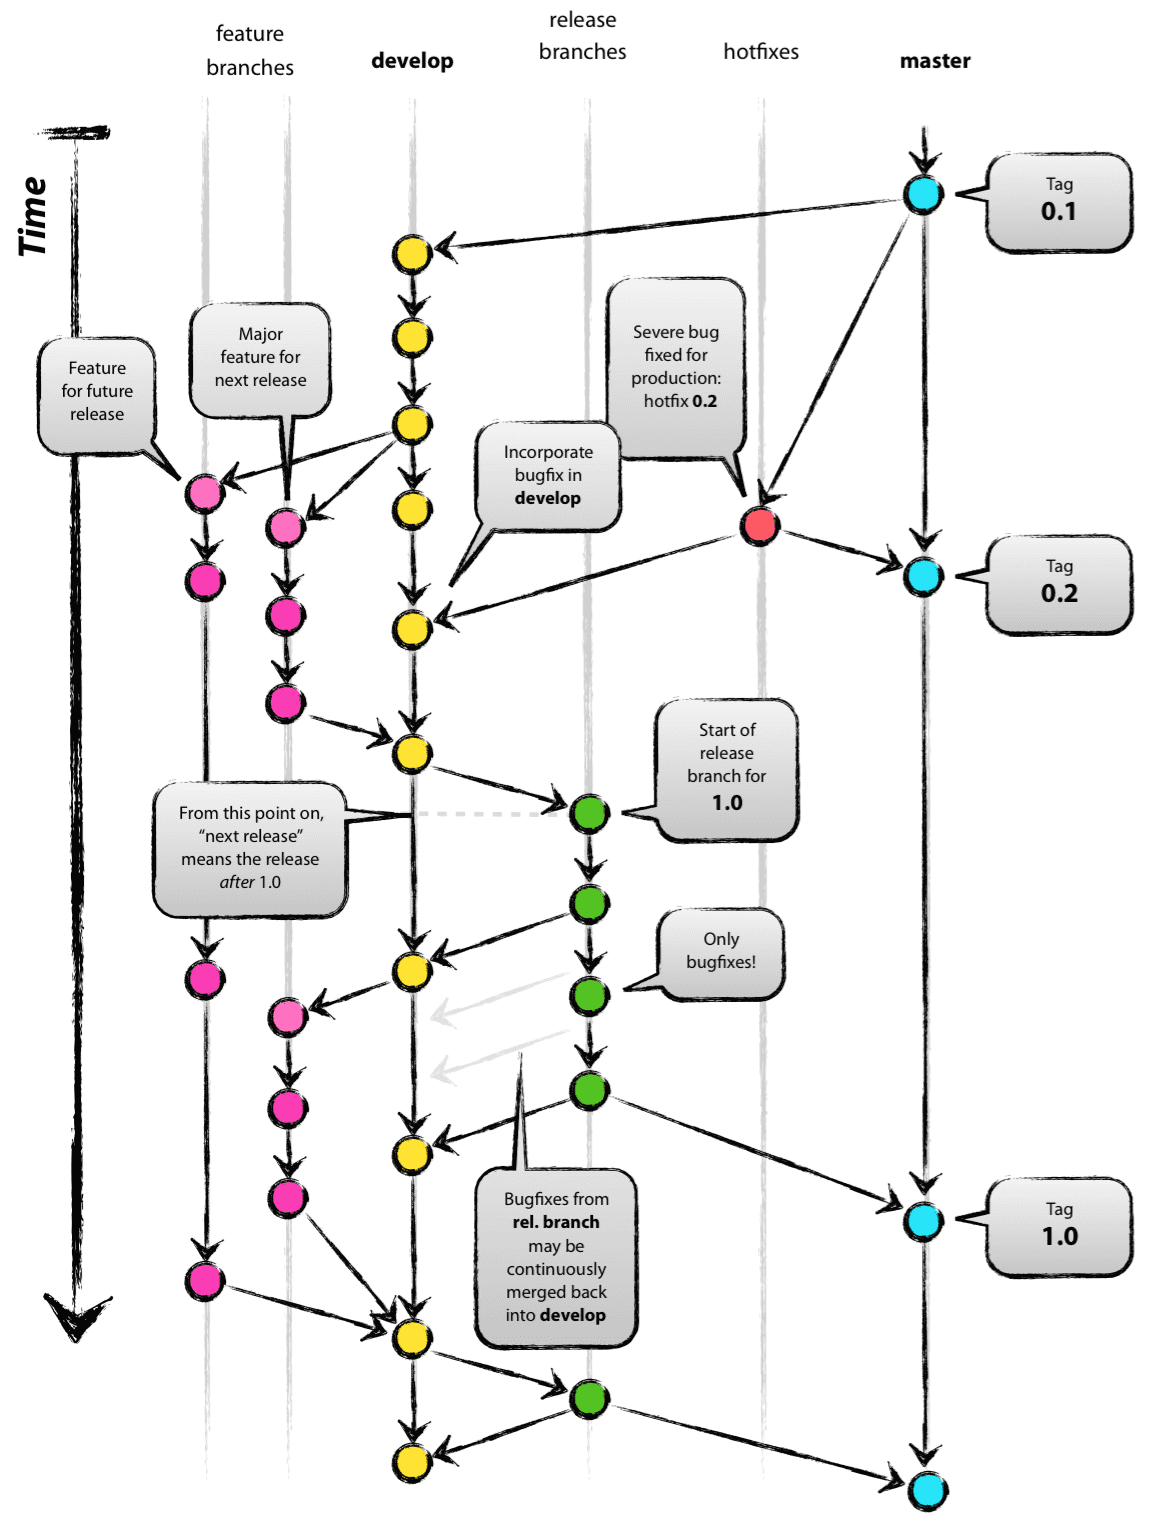
\includegraphics[width=0.9\textwidth]{gitflow.png}
 \bicaption[fig:longcaptionbad]{Git-flow 工作机制示意图}{Git-flow 工作机制示意图}{Fig}{Git-flow working mechanism}
\end{figure}

Git-flow管理的项目仓库中有两个主要的分支:主分支(master branch)和开发分支(develop branch),分别对应正式生产环境\footnote{正式给用户使用的环境}和测试环境\footnote{给测试人员测试和测试用户熟悉系统的环境};另外还有一些辅助分支:新特性分支(feature branches)、预发布分支(release branches)和热修复分支(hotfix branches),其中新特性分支对应新特性测试环境\footnote{专为新特性测试单独部署的环境,数据与测试环境相同},其余两个对应准生产环境\footnote{专为发布之前和热修复测试单独部署的环境,数据与生产环境相同}。

如图2-3所示,竖直向下的轴是时间轴,横轴是不同的分支,图上的圆圈圈住的点表示发生在不同时间的不同的提交(Commit),带有箭头的线表示提交的父子关系,箭头来自的提交是箭头指向的提交的父亲\footnote{Git中的提交允许有多个父提交和多个子提交}。本课题将从时间顺序剖析这张图来介绍Git-flow的工作机制,假设开发人员甲负责新特性开发,开发人员乙负责修复发布和BUG,任何人都可以维护开发分支
\begin{enumerate}
  \item 故事从任何一次发布之后开始,主分支上带有0.1标签(Tag)的是最早的一个提交,“Tag0.1”标志着刚刚经过了一次正式发布;
  \item 发布完成之后,开发人员先把主分支合并到开发分支,产生了一个提交,然后可能做了两个影响不大的微小调整(两个新的提交);
  \item 这时开发人员甲从开发分支分出了一个早就想做但不是很急的特性分支,我们把它叫做“未来特性”(Feature for future release);
  \item 紧接着产品经理说有一个加急特性要加上,于是开发人员A暂且放下“未来特性”的工作,又从开发分支分出了第二个特性分支,暂且叫做“下一个特性”(Major feature for next release),这是一个典型的多特性并行开发的情况;
  \item 与此同时生产环境可能发现了一个bug,开发人员乙从主分支分出一个热修复分支0.2,修复完bug后先合并到了主分支打上标签0.2,再合并到了开发分支,在开发分支上产生了一个新的提交(Incorporate bugfix in develop);
  \item 又过了一段时间,开发人员甲完成了“下一个特性”,合并到了开发分支上,回头继续开发“未来特性”;
  \item 开发人员乙从develop分出了一个预发布分支1.0,部署到准生产环境,经过开发人员的测试发现了一个bug,开发人员乙修复并合并回了开发分支;
  \item 这时产品经理说又有一个新特性要加上,但打算和“未来特性”一起发布,于是开发人员甲又从开发分支分出一个新特性分支并同时开发这两个新特性;
  \item 开发人员乙在预发布分支1.0上面又修复了后来发现了几个bug,其中有几次反复地合并回了开发分支,为了其他开发人员能更好地开发;
  \item 到了正式发布的时机了,开发人员乙把预发布分支先合并到了开发分支,再合并到了主分支,并在主分支上打上标签1.0;
  \item 然后开发人员甲完成了两个新特性,开发人员乙又发布了一次,虽然图上没有,但之后应该会再把主分支合并到开发分支;
\end{enumerate}

本系统开发过程中统一使用了Git-flow来管理分支,如图2-4所示,Azwraith项目在4月21日到26日之间的表现就比上图更加复杂,但仓库管理过程依然方便快捷。其中黑线是主分支,紫色线是开发分支。

\begin{figure}[!htp]
 \centering
 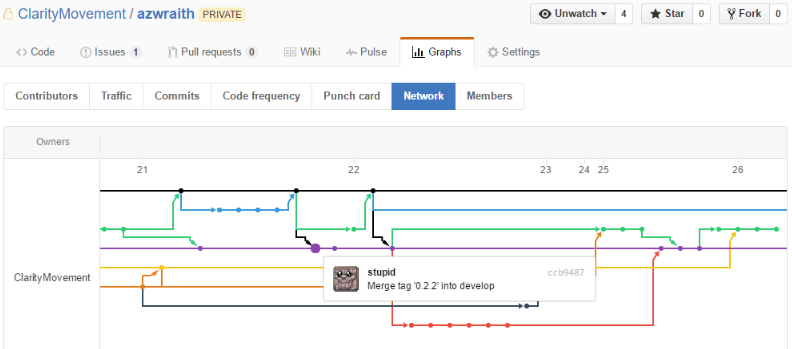
\includegraphics[width=0.99\textwidth]{azwraith_network.png}
 \bicaption[fig:longcaptionbad]{Azwraith 分支网络}{Azwraith 分支网络}{Fig}{Azwraith branch network}
\end{figure}

\subsection{IDE&文本编辑器: Webstorm VS Atom}
Webstorm 是JetBrains公司开发的一系列集成开发环境(IDE)中面向JavaScript的一款收费桌面应用。JetBrains公司在像Java这样的静态语言语法分析方面经验丰富,像JavaScript这样的非静态语言也处理的非常好。
Atom是一个由Github开发的一款免费的开源的文本和源代码编辑器,面向OS X、Linux和Windows用户,支持用NodeJS编写的插件并且内置了Git版本控制。Atom也有一个强大的社区维护者免费的扩展包。
本系统开发过程中,只在版本管理模块的前端使用了Atom,其他部分均使用了Webstorm。因为Atom比较轻量级并且Atom的社区提供的各种扩展可选择性很强,最重要的一点是AngularJS使用的是依赖注入,不像ReactJS和NodeJS有大量的模块互相引用,因此不需要IDE有很强的项目文件关系处理和跨文件变量解析能力。

\subsection{代码生成: Yeoman和Yeoman Generators}
Yeoman是一个开源的客户端开发工具,包括一系列帮助开发人员搭建WEB应用程序的工具和框架。Yeoman运行起来是一个命令行交互界面,工具开发人员利用它来和应用开发人员交互(或者不进行交互)获取一些信息后运行用NodeJS写的一些功能函数,如生成一个WEB应用程序的启动模板、管理依赖、运行单元测试、提供一个本地开发服务器和优化生产环境代码等。

generator-material-app\footnote{\url{https://github.com/michaelkrone/generator-material-app}}是一个生成Material Design风格的MEAN应用脚手架(基本框架)的Yeoman代码生成器。

本系统在开发时,主要是版本管理模板因为是一种比较成熟的后台管理系统,使用了代码生成器来生成初始的结构和开发过程中的模块,这极大地减少了重复劳动,增加了代码可维护性,解放了开发人员的生产力。


\subsection{构建工具: Grunt VS Gulp VS Npm}
构建工具是用来构建各种自动化任务的工具,比如编译、测试等操作,有些需要一系列复杂的指令或者逻辑,那么就可以用构建工具来构建一个“自动化任务”,之后只要用这个构建工具来运行这个任务,就能完成这项操作。现在JavaScript世界主要使用3种主流的构建工具grunt、gulp和npm:
\begin{description}
  \item[grunt] 使用基于声明式配置的配置文件来定义任务,自定义插件、社区强大、简单易用,不需要任何高级的概念或知识。但由于它基于配置,一旦任务数量多了或者复杂了,grunt配置文件将会变得特别复杂而且难以控制任务执行的顺序。
  \item[gulp] 使用基于流处理的JS代码来定义任务,设计之初就是想要取代grunt,自定义插件、可扩展性强、只需要了解JavaScript就可以自定义任务,和grunt一样依然依赖插件和插件作者。
  \item[npm] 使用NodeJS和bash脚本来定义任务,不依赖插件和插件作者,可扩展性最强,自由度最高,但需要熟悉NodeJS和bash脚本。
\end{description}

这三种构建工具从上到下,使用难度增大、可扩展性变强、自由度变高。本系统在选择构建工具时颇有一番斟酌,最终考虑到npm的难度,在大部分系统中使用了gulp来构建,只在Smart City模块的前端使用了npm以作试点。

\subsection{代码质量}
代码质量指的是软件的结构性质量,包含一些与功能需求无关的代码如何组织、软件是否正确生产的特性,如可读性、健壮性和可维护性。

本小节介绍了一系列提高代码质量的手段和工具:代码风格指南、代码风格检查器、Git钩子机制(Git hooks)和代码审查(code review)。其中后者是前者的保障或备案。
\subsubsection{代码风格指南: John Papa和Airbnb}
风格指南(style guide)是一种编写和设计文档的标准集,不管是大众用途的还是某一个特殊领域的,比如代码编写。遵从统一的代码风格指南可以提高代码的一致性从而提高代码的可读性,一个代码风格指南一般是由一些权威的人士或者公司总结了一些最佳实践(Best practice)来编写出来的,所以能够提高代码质量,避免或减少常见错误。

本系统中使用了两种风格指南,一个是AngularJS的比较权威的“John Papa的风格指南”\footnote{\url{https://github.com/johnpapa/angular-styleguide}}(John Papa's Styleguide),另一种是ReactJS和NodeJS的“Airbnb\footnote{美国一家做租房的公司,相当于租房业的Uber}风格指南”\footnote{\url{https://github.com/airbnb/javascript}}。

当然风格指南只是一种指南,并不能保证每个开发人员至始至终遵守,人也没有精力准确地判断梅一段代码是否符合风格指南,还需要一些工具来保证代码的风格一致性。
\subsubsection{代码风格检查器: JSCS、 Jshint/ Eslint和Stylelint}
检查代码风格的一个主要工具是各种代码风格检查器,以下列出本系统中使用的各类地代码风格检查器:
\begin{itemize}
  \item JSCS是一种针对JavaScript的语法层面的代码风格检查器,并有一定的自动修复功能,没有默认的规则要求,就是说如果不指定规则,JSCS什么都不会检查。
  \item Jshint是一种针对JavaScript的语法及语义层面的代码风格检查器,一般与JSCS混合使用,专注检查语义,有一些默认的规则要求。
  \item Eslint和Jshint类似,有着最好的ES6支持,一般也与JSCS混用,有一些默认的规则要求。
  \item Stylelint是一种针对CSS的代码风格检查器,没有默认的规则要求。
\end{itemize}

这些代码风格检查器都通过一个简单的配置文件\textbf{.jscsrc、.jshintrc、.eslintrc、.stylelintrc},里面列有一系列的规则来自定义想要的各种代码风格。也可以通过简单的preset选项来使用某一个内置的代码风格,然后可以增加一些规则来修饰。如果在某一个单独的文件中想要突破规则也可以暂时地修改规则或者关闭规则。

这里以JSCS为例,本系统在使用“John Papa的风格指南”时是完全自己定义,因为太长所以不在这里展示,而在使用“Airbnb代码风格”时使用的是preset选项再加上一些自己的修改:
\begin{lstlisting}[language={JSON}, caption={Airbnb代码风格JSCS配置}]
{
  "preset": "airbnb",
  "esnext": true,
  "excludeFiles": ["build/**", "node_modules/**"],
  "validateQuoteMarks": null,
  "requireCurlyBraces": ["else", "for", "while", "do", "try", "catch"]
}
\end{lstlisting}

虽然在这里都罗列出来介绍,但其实Jshint和Eslint是可选的,AngularJS不需要ES6支持,所以在版本管理模块中使用了Jshint,而且其他两个模块中使用了Jshint。

有了代码质量检查器也不能保证开发人员会去使用,或者开发人员是同意使用的,但总是会有忘记和疏漏的时候。这时就需要Git hook来保障代码质量检查器的运行。
\subsubsection{Git hooks 和 Pre-commit}
Git hook是Git提供的一种钩子(hook)机制,每当你使用Git做某种操作时就会触发来执行一段脚本,比如本系统中就是用了\textbf{预提交钩子(pre-commit hook)},顾名思义就是在提交之前会执行的钩子。

本系统中使用了一个开源的封装\textbf{pre-commit},配合npm脚本(scripts)只需要安装和在\textbf{package.json}中简单的配置就能在每次commit之前运行我们的代码风格检查器:
\begin{lstlisting}[language={JSON}, caption={package.json中的pre-commit设置部分}]
{
  "...": "...",
  "scripts": {
    "eslint": "eslint src tools",
    "jscs": "jscs src tools --verbose",
    "stylelint": "stylelint 'src/**/*.scss' --syntax scss"
  },
  "pre-commit": [
    "eslint",
    "jscs",
    "stylelint"
  ]
}
\end{lstlisting}

然而Git又提供了一些方法来突破钩子机制直接提交,毕竟有可能会发生恶意篡改代码风格检查器配置或者没空修复代码风格的紧急情况,所以Git hook也不是最终的保障。
\subsubsection{Code review}
一台机器可以做五十个普通人的工作,但是没有哪部机器可以完成一个伟人的工作\supercite{hubbard2015one}。最终的检查还是要靠人,代码审查(code review)是一种对软件源代码的系统性检查,目的是找出在开发阶段倍忽视的错误和提高整体的代码质量。代码质量经常能够发现一些常规的安全漏洞来提高软件的安全性,如格式字符串漏洞、竞争情况、内存泄漏和缓冲区溢出等。在线代码仓库如git、svn\footnote{类似git的一个版本控制系统}等允许团队协作地进行代码审查。

本系统在开发过程中,把代码审查和前文提到的Git flow结合,每个新特性分支、热修复分支和预发布分支在合并到主要分支之前,都需要先发出一个合并请求(git上叫做pull request),然后指定团队中的一个人从客观的角度审查每一行修改,如果新增的代码或改动能让一个不够了解这个项目、这个特性的人也能看懂其意图,那么证明它的可读性和可维护性是足够高的,从而保障了主要分支代码的高质量。
\subsection{单元测试: Karma、 Mocha、 Chai 和 Sinon}
Karma是AngularJS开发团队研发的一个专门用于跑测试的系统,主旨在于给开发者提供有生产力的(productive)测试环境。开发人员不需要设置复杂的配置载入,只需要写测试、写代码然后获得及时的测试反馈,这样开发人员才能够既有生产力(productive)又有创造力(creative)。

Mocha是一款功能全面的测试框架,既能在NodeJS中运行也能在浏览器中运行,能够很好地支持异步测试。Mocha串行地执行测试程序,给出灵活切准确的报告,而且能够把未捕捉到的异常映射到正确的测试用例上面。

Chai是一个测试驱动开发(TDD)或行为驱动开发(BDD)的断言库或者叫语言库,它运行在NodeJS或者浏览器中,可以轻易地与各种JavaScript测试框架结合。链式的BDD风格(包括should和expect两种风格)提供了富有语言表现力和可读性的代码:

\begin{lstlisting}[language={JavaScript}, caption={BDD风格的chai代码}]
foo.should.be.a('string');
foo.should.equal('bar');

expect(foo).to.be.a('string');
expect(foo).to.equal('bar');
\end{lstlisting}
而TDD的断言风格给人一种经典的感觉
\begin{lstlisting}[language={JavaScript}, caption={像自然语言一样的测试代码}]
assert.typeOf(foo, 'string');
assert.equal(foo, 'bar');
\end{lstlisting}

Sinon是一个独立的与测试框架无关的JavaScript,专注于做间谍(spy)\footnote{包装过的类或者对象,拥有正常的行为,但每一个动作都被监听}、桩(stub)\footnote{假的类或者对象,直接模拟一些指定的行为,给出特定的、看起来正确的结果}和模(mock)\footnote{完全的假的类或对象,任何行为直接返回0或者空}。

本系统中的单元测试使用Karma作为测试环境,Mocha作为测试框架,BDD风格的Chai作为测试语言,使用Sinon来模拟家的JavaScript对象和函数。
\subsection{持续集成: Solano CI}
Solano CI是一个持续集成和部署解决方案。可以直接使用在线的SaaS云服务,也可以在私有虚拟设备上搭建主机。Solano CI独有的时间表(schedule-optimizing)优化技术使用测试文件的多重输入来计算最好的运行时间,使其能够自动地、智能地并行执行自动化软件测试。开发人员只需要简单的配置就能够轻松地完成持续集成和自动部署,本系统中的持续集成使用情况会在后面的专门章节介绍。


